\chapter{机器学习概述与数据特征工程}
\section{引言}
从本章起,本研究将使用机器学习的一般方法对PE患者及正常妊娠孕妇的脉搏波数据进行相关分析研究。
作为过渡章节,本章首先进行了机器学习的一般概述,介绍了机器学习的一般步骤与流程,并明确本研究的机器学习任务。特别地,
在机器学习开始之前,一般还需对使用的数据进行额外的处理工作,即数据特征工程,本章也对这部分的工作内容进行了相应的介绍。

\section{机器学习概述}
本小节将从机器学习的基本概念、分类、一般步骤流程及本研究涉及的机器学习任务等方面进行介绍。
由于篇幅内容所限,机器学习领域常见的术语并没有在正文中过多提及,部分术语及其解释可参见本文末附录D。
\subsection{机器学习简介}
一般认为,机器学习是一门致力于研究通过计算的手段、利用已有的经验来改善系统自身性能的学科(和艺术)\cite{Zhou2016,Aurélien2018}。其中,Tom Mitchell对机器学习给出了一种最为经典的形式化定义:
计算机程序利用经验$E$学习任务$T$,其性能是$P$,如果针对任务$T$的性能$P$随着经验$E$不断增长,那么我们就说关于$T$与$P$,该程序对$E$进行了学习,这一过程如\autoref{fig:etp}所示\cite{mitchell1997,Zhou2016}。
对计算机程序而言,$E$通常以数据的形式存在,因此机器学习也可以看成从相关数据中产生模型的算法过程,不显式编程是机器学习最典型的特征。
\begin{figure}[htbp]
  \centering
  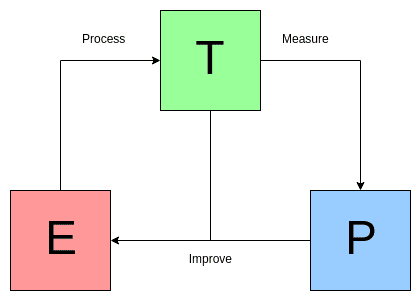
\includegraphics[width=.5\linewidth]{features/etp}
  \caption[机器学习方法的形式化定义]{\label{fig:etp}机器学习的形式化定义}
\end{figure}

尽管机器学习的相关概念早在上世纪五十年代就已经被提出,但直到进入新世纪后,机器学习才真正迎来井喷式发展的黄金期。在过去二十年中,由于半导体电子计算机行业的充分发展,人类收集、传输、处理数据的能力取得了长足的进步,
人类各种社会活动中出现的海量数据具备了能够被挖掘、分析的硬件基础与需要被分析并加以利用的客观需求。在此背景下,机器学习受到了学者们的广泛关注并进入了蓬勃发展阶段,不论是理论基础方面亦或是应用研究方面都
得到了巨大的发展,取得了重大突破。目前,机器学习技术已经被成功应用在模式识别、数据挖掘、自然语言处理、语言识别、图像识别、芯片设计、信息检索及生物信息学等学科领域,
尤其是为交叉学科的发展研究提供了新的技术支撑与突破点\cite{Zhou2016,Aurélien2018,Li2017}。

\subsection{机器学习的分类}
尽管有多种分类标准,基于机器学习在学习阶段呈现的输入数据与预期输出之间的潜在映射关系可将机器学习归纳为以下几类\cite{awad2015,Li2017,Aurélien2018}:

一、监督学习

监督学习是一种用于推断观察数据(也称为输入数据)与目标变量(因变量或标签)之间的潜在关系的学习机制。
学习任务使用标记的训练数据(训练示例)来合成模型函数,这些模型函数的目的是概括特征向量(输入)和监控信号(输出)之间的基本关系。
训练数据包括观察到的输入(特征)向量和期望的输出值(也称为监控信号或类别标签)。基于监督学习算法的经过良好训练的函数模型可以准确预测隐藏在不熟悉或未观察到的数据实例中的隐藏现象的类标签。

二、无监督学习

无监督学习算法被设计用于发现未标记数据集中的隐藏结构,其期望输出是未知的。
一般而言,无监督学习的数据集仅由数据特征集$x_1,x_2,\dots,x_n$组成,没有监督学习中的目标输出,也不包含任何环境激励回报。
聚类与降维是无监督学习两个最为流行的应用方向。此外,无监督学习机制在数据压缩、离群点检测、分类、人类学习等领域均有着广泛应用\cite{awad2015}。

三、半监督学习

半监督学习使用少量标记数据集和大量未标记数据集的组合来生成模型函数或分类器,是监督学习与无监督学习两种机制的结合。
随着海量数据的涌现,对原始数据集的标记过程往往需要大量的人力成本、时间成本,直接对这些数据进行监督学习无疑是不明智的。
而半监督学习正是以未标记的数据为基础,综合应用无监督学习(大量未标记的训练数据)和监督学习(少量标记的培训数据)两种机制,可以显著提高学习精度。
半监督学习目前已在网络数据、消息数据、股票数据、零售数据、生物数据、图像等领域得到应用,特别是在与人类学习相关的语音、视觉和手写识别等领域\cite{awad2015,Aurélien2018}。

四、强化学习

强化学习是通过给定的一组实验动作和观察到的对环境状态的响应进行训练来合成适应模型的过程。
这种方法可以被视为一种控制理论的试错学习范式,其学习系统(在其语境中一般也称为智能体)能够观察环境,做出选择,执行操作,并获得回报或惩罚。
为最大化累计奖励,强化学习的智能体必须自主学习什么是最好的策略。
强化学习在信息论、博弈论、自动控制等领域均得到应用。近年来大热的阿尔法围棋(AlphaGo)就是强化学习最为典型的应用之一\cite{Silver2016}。

五、转换学习

转换学习(又称转换推理)试图通过使用与新案例相关的训练数据集上的额外观察来预测特定测试案例上的排他性模型函数。
转换学习通过将新的个体观测(训练数据)拟合到空间中的单个点来建立局部模型而非全局模型,在给定问题空间出现不连续时有着极佳的发挥空间,可以在不连续边界合成多个模型\cite{Silver2016}。

\subsection{本研究的机器学习任务}
\autoref{fig:spml}展示了一个完整的监督学习工程的处理逻辑,主要包含以下步骤\cite{Aurélien2018}:

一、提出具体问题

针对具体情景,明确需要解决的问题及研究目标。

二、数据特征工程

数据特征工程主要包含数据获取、研究数据特性及处理缺失值、标准化等在内的数据准备等内容。

三、训练模型

基于数据探索多种机器学习模型,列出解决问题的最佳模型,对这些模型的超参数进行调整,优化最佳模型。

四、结论与演示

系统地概括总结问题,展示最终解决方案,展示(并解释)以上过程中所出现的现象及问题。

五、生产与部署

准备好最终解决方案的生产环境并进行部署,对系统性能进行监测并定期重新建模等。
\begin{figure}[htbp]
  \centering
  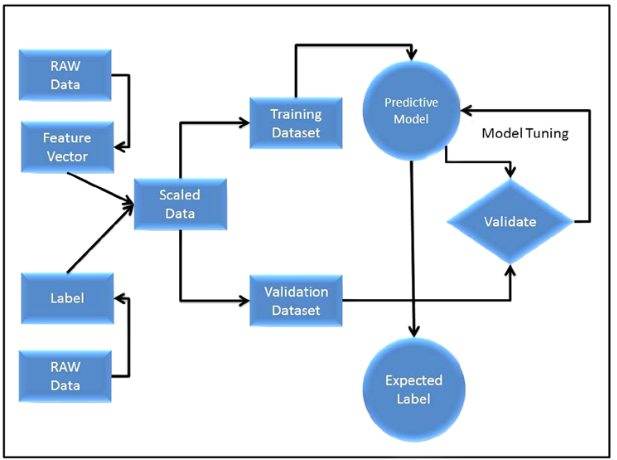
\includegraphics[width=.6\linewidth]{features/spml}
  \caption[监督学习的处理逻辑]{\label{fig:spml}监督学习的处理逻辑\cite{awad2015}}
\end{figure}

回归到本研究的工作内容上来,不难发现,\textbf{探求子痫前期与孕妇脉搏波波形之间的潜在关系}是本研究要具体探索解决的关键性问题。
本文后续内容即为综合应用\textbf{监督学习}与\textbf{无监督学习}的相关算法按上述步骤解决该问题的过程。其中,所有处理程序均在Python环境(Python 3.9.7, 64 bit)下开发完成,
综合使用了Pingouin、Scikit-learn、DESLib及TensorFlow等开源组件工具\cite{python,Vallat2018,scikit-learn,JMLR:v21:18-144,tensorflow2015-whitepaper}。

\section{数据特征工程}
数据特征工程是对原始数据进行一系列工程处理并将其提炼为特征作为输入供算法和模型使用的过程\cite{Zhou2016,Aurélien2018}。
特征工程的核心是表示与展现数据,其本质是去除原始数据中的杂质和冗余,设计更高效的特征以刻画求解的问题与预测模型之间的关系。
下面将对本研究涉及的特征处理进行说明与介绍。

\subsection{数据集构建}
第三章已经对脉搏波的描述特征参数进行了介绍,本研究选取了其中的部分参数构成了基本输入数据集。实际上,本研究共构建了三类脉搏波描述特征集。

一、

* 分析数据集准备:两种方式

  * A. by pulse

  * B. by person
\subsection{PPG时域描述特征集构建}

本小节对本研究实际采用的多种PPG时域描述特征进行汇总,对各参数符号及前置计算条件也进行了统一说明,如\autoref{tab:allfeatures}所示。
TODO
\begin{center}
    \fontsize{10}{4}
    \begin{longtable}{p{3cm}<{\centering}p{1cm}<{\centering}p{2cm}<{\centering}p{6cm}<{\centering}p{1cm}<{\centering}}
        \caption{本研究使用的所有PPG时域指标一览}\\
        \label{tab:allfeatures}\\
        \hline\hline
            \textbf{研究者}&\textbf{时间}&\textbf{脉搏波参数}&\textbf{研究结果}&\textbf{备注}\\
        \hline
        \endfirsthead
        \caption[]{(续)}\\
        \hline
            \textbf{研究者}&\textbf{时间}&\textbf{脉搏波参数}&\textbf{研究结果}&\textbf{备注}\\
        \hline
        \endhead 
        \hline
        \endfoot
        \hline\hline
        \endlastfoot
        &       &       &       &  \\
        &       &       &       &  \\
        &       &       &       &  \\
        &       &       &       &  \\
        &       &       &       &  \\
    \end{longtable}
\end{center}
\subsection{两种划分方式}
\subsection{数据集的处理}

\subsection{数据清洗}
* 处理缺失值

\subsection{新特征的创建}
* 构建新特征(char参数)
\subsection{相关性验证}
* 分布特性

  * 有无差异性,SPSS统计,已用python实现

  * 特征相关性,heatmap
\subsection{特征缩放}
* 标准化
\subsection{特征降维}
* 降维与特征贡献度

* 部分工作需要下一章节完成后才能确认
\section{小结}